\chapter{Data Link Layer}\label{sec:datalink_intro}
Well! We've finally made it past the Physical Layer, which is a good thing, because it can be pretty boring. The Data Link Layer is where things start to get interesting, as it is the first layer that deals with actual data packets and their transmission over a physical medium.

\section{tl;dr}
The Data Link Layer is the second layer of the OSI model, sitting above the Physical Layer and below the Network Layer. It provides node-to-node\footnote{
    directly connected devices, \textbf{not} end-to-end communication!!!
} data transfer and handles error correction from the Physical Layer. The Data Link Layer is responsible for framing, addressing, and error detection and correction.

It's further divided into two sublayers - the Logical Link Control (LLC) and the Media Access Control (MAC). The LLC sublayer is responsible for managing communication between devices, while the MAC sublayer handles access to the physical medium. 

If you were to run \texttt{ifconfig} on a Linux machine, you would see the MAC address of your network interface card (NIC) listed under each interface\footnote{
    Interfaces are the logical representations of your network connections, such as Ethernet or Wi-Fi. It is not tied to hardware, but rather to the software that manages the hardware. There exist virtual interfaces as well, which are used for things like VPNs and Docker containers.
}'s \texttt{ether} field.

\begin{verbatim}
$ ifconfig
wlan0: flags=4163<UP,BROADCAST,RUNNING,MULTICAST>  mtu 1500
    inet 10.0.0.100  netmask 255.255.255.0  broadcast 10.0.0.255
    inet6 fe80::f00d:dead:1337:d00d  prefixlen 64  scopeid 0x20<link>
    ether f0:0d:de:ad:13:37  txqueuelen 1000  (Ethernet) <---- MAC address
    RX packets 80085  bytes 5551234 (5.5 MB)
    TX packets 31415  bytes 2718281 (2.7 MB)
\end{verbatim}


% collisions
\section{Collisions}\label{sec:collisions}
Continuing from the previous section (\ref{subsec:carriers_sensing}), we now turn our attention to one of the challenges of networking: collisions. 

A collision happens when two or more devices decide to "speak" (transmit data) at the exact same time over the same communication channel. You can imagine why that's problematic. The most common way of dealing with this is to either detect the collision and retransmit the corrupted data or to avoid the collision altogether.

Collisions come in various ca;ibers - partial corruption affects only portions of data, full destruction where entire frames are lost. A particularly interesting case is the hidden terminal problem, where two devices can't detect each other's presence but attempt to communicate with the same destination simultaneously. We'll explore this phenomenon later in the chapter.

Your network interface card (NIC) constantly manages these collision scenarios, implementing detection and recovery mechanisms to maintain reliable communication.
\vfill
% /assets/diagrams/csma/collisions.png
\begin{figure}[h]
    \centering
    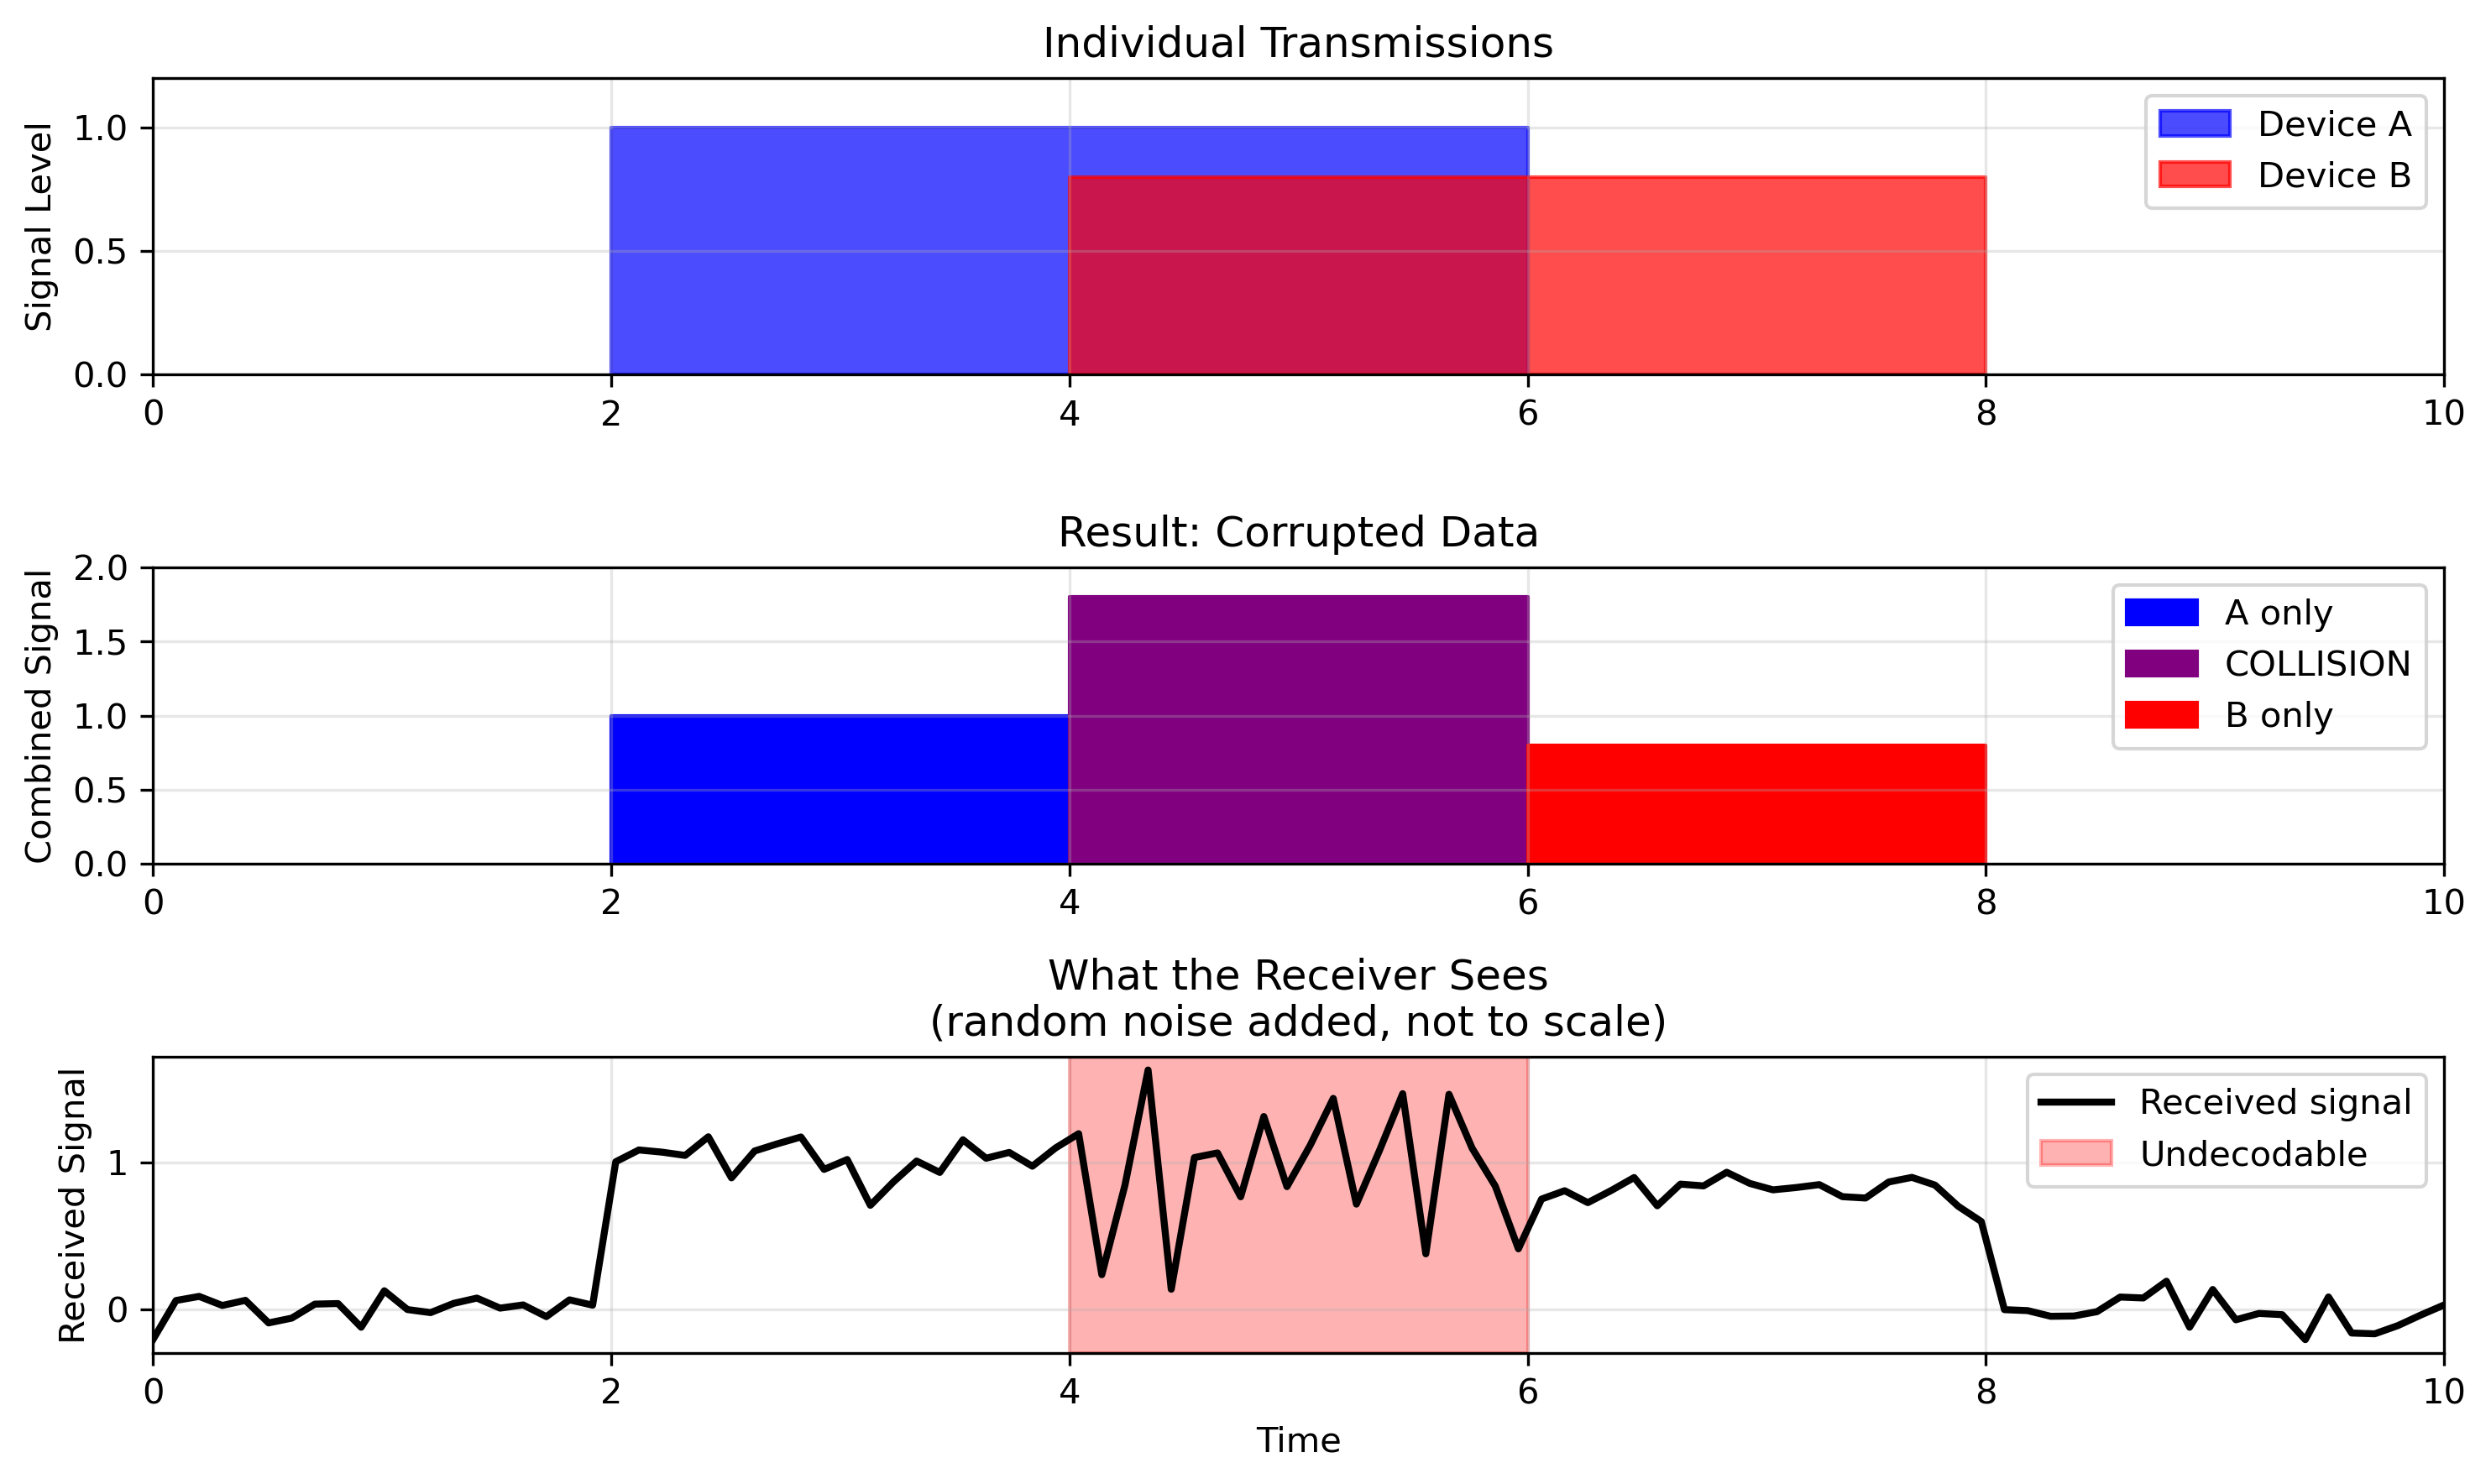
\includegraphics[width=\textwidth]{assets/diagrams/csma/collisions.png}
    \caption{Example of a collision}
    \label{fig:collision_visualization}
\end{figure}

\newpage
\subsection{Carrier Sense Multiple Access (CSMA)}
Now that we understand the problem, let's understand one of the solutions.

CSMA works on a simple principle: before transmitting anything, a device listens to the channel to see if anyone else is already talking (carrier sensing). If the channel is free, it goes ahead and transmits. If someone else is already using the channel, it waits for its turn (busy waiting).

\begin{figure}[h]
    \centering
    \scalebox{0.7}{\input{assets/diagrams/csma/normal.latex}}
    \caption{CSMA Flowchart}
    \label{fig:csma-normal}
\end{figure}

\subsubsection{+ Collision Detection (CSMA/CD)}
CSMA/CD introduces real-time collision detection. The only difference from the barebones version is that while transmitting, devices continue listening to the channel. If they detect that their signal has been corrupted by interference (collision), they immediately stop transmitting and implement a "backoff" strategy.

The backoff algorithm uses exponential backoff, meaning that after multiple failed attempts, devices wait progressively longer before retrying. This prevents starvation\footnote{
    Starvation is a scheduling problem where a process is perpetually denied the resources it needs to proceed, often due to other processes monopolizing those resources or the algorithm causeing it to wait indefinitely.
}.
\subsubsection{+ Collision Avoidance (CSMA/CA)}
As the name implies, CSMA/CA tries to avoid colissions entirely.

The protocol uses a handshake mechanism called RTS/CTS (Request to Send/Clear to Send).

\speechleft{Device A}{"May I please transmit to Device C?" (RTS)}
\speechright{Device C}{"Yes, go ahead, I'm ready to listen" (CTS)}
\begin{tcolorbox}[colback=gray!10, colframe=gray!50, arc=3mm, left=2mm, right=2mm, boxrule=1pt, before skip=5mm, after skip=5mm]
    \textit{Other devices hear this exchange and know to stay quiet during the upcoming transmission}
\end{tcolorbox}
\speechleft{Device A}{\textit{Transmits data with confidence}}

You'll notice how prevalent this type of conversation (protocol design) is in networking. ACKs and NACKs and handshakes are everywhere! Network people have found that this approach works well and provides much needed structure to the communication process.

\subsection{Persistence}
You might also be wondering how long a device should wait before trying to transmit again after a collision or when the channel becomes free. I guarantee you that this is something you have already thought about, but this is just about putting a name to it. 


\subsubsection{1-Persistent CSMA}
In 1-persistent CSMA, when a device finds the channel busy, it continuously monitors the channel and transmits immediately when it becomes free. This is the most aggressive approach - devices are "persistent" with probability 1.

While this minimizes delay when the channel becomes available, it also maximizes the probability of collisions when multiple devices are waiting. If two or more devices are listening to a busy channel, they will all attempt to transmit simultaneously once it's free.

\subsubsection{Non-Persistent CSMA}
Non-persistent CSMA takes the opposite approach. When a device finds the channel busy, it waits for a random amount of time before checking again, rather than continuously monitoring.

This reduces the collision probability since devices don't all rush to transmit at the exact moment the channel becomes free. However, it can lead to wasted channel capacity - the channel might sit idle while devices are in their random wait periods.

\subsubsection{p-Persistent CSMA}
p-persistent CSMA offers a compromise between the two extremes. When the channel becomes free, each device transmits with probability \textit{p}, or waits until the next time slot with probability \textit{(1-p)}.

The value of \textit{p} can be tuned based on network conditions - lower values reduce collisions but increase delay, while higher values do the opposite. This approach is commonly used in slotted networks where time is divided into discrete slots.

% /assets/osi/datalink/csma/persistence.png
\begin{figure}[h]
    \centering
    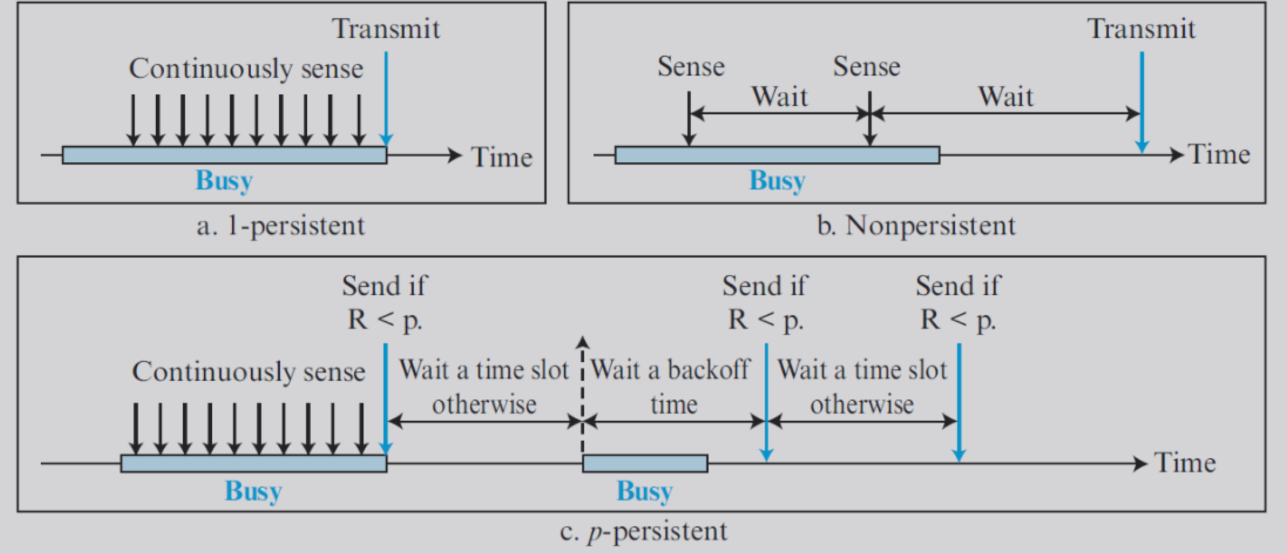
\includegraphics[width=.8\textwidth]{assets/osi/datalink/csma/persistence.png}
    \caption{Persistence in CSMA}
    \label{fig:csma-persistence}
\end{figure}
% framing
\section{Framing}\label{sec:framing}
When you need to send data over a network, you can't just throw it out there and hope for the best (unless you're UDP, which does exactly that). You need to package it up in a way that makes sense to the receiving device. This is where framing comes into play.

Framing is the process of encapsulating data into discrete units called frames. Each frame contains not only the actual data being sent but also additional information that helps the receiving device understand how to process it. This includes things like source and destination addresses, error-checking information, and control information. We'll go through some frame structure diagrams \textit{a lot} in this reader, so get used to it!

\section{Ethernet}
\label{sec:ethernet}
Ethernet is the most widely used local area network (LAN) technology today. It defines both the physical layer specifications (cables, connectors) and the data link layer framing protocol.

\subsection{Ethernet Frame Structure}
Remember when I said you should get used to frame structure diagrams? Well, here's one for Ethernet:

\begin{figure}[h]
    \centering
    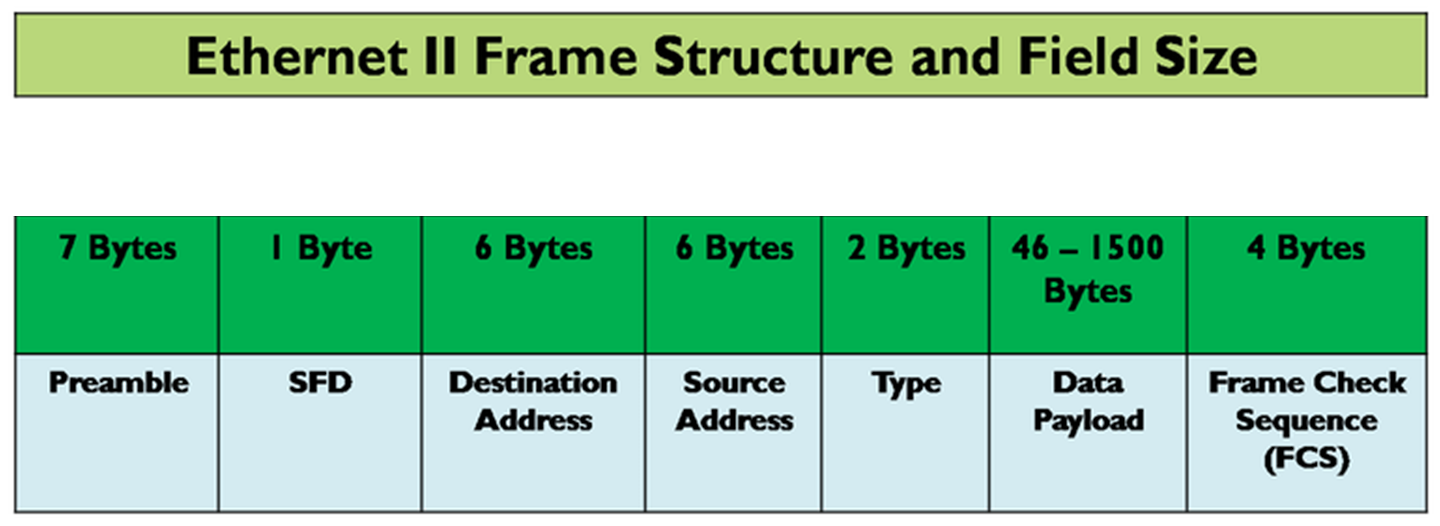
\includegraphics[width=\textwidth]{assets/osi/datalink/protocols/ethernet.png}
    \caption{Ethernet Frame Structure}
    \label{fig:ethernet_frame_structure}
\end{figure}

\begin{itemize}
\item \textbf{Preamble (7 bytes):} A sequence of alternating 1s and 0s used for synchronization
\item \textbf{Start Frame Delimiter (1 byte):} Marks the beginning of the frame with pattern 10101011
\item \textbf{Destination Address (6 bytes):} MAC address of the receiving device
\item \textbf{Source Address (6 bytes):} MAC address of the sending device
\item \textbf{Type/Length (2 bytes):} Indicates either the protocol type or frame length
\item \textbf{Data (46-1500 bytes):} The actual payload being transmitted
\item \textbf{Frame Check Sequence (4 bytes):} CRC-32 checksum for error detection
\end{itemize}


Different Ethernet standards may have variations in frame size and structure, but the basic components remain consistent. The minimum frame size is 64 bytes, and the maximum is 1518 bytes (or 1522 bytes with VLAN tagging).

\newpage
There are different physical specifications as well, which you will never need in real life, but might come across on the exam. If you need a refresher on the different types of cables, check out Section \ref{sec:transmission_media}.

\begin{table}
    \centering
    \begin{tabular}{|c|c|c|}
        \hline
        \textbf{Ethernet Standard} & \textbf{Speed} & \textbf{Cable Type} \\
        \hline
        10BASE-T & 10 Mbps & Twisted Pair (Cat 3) \\
        100BASE-TX & 100 Mbps & Twisted Pair (Cat 5) \\
        1000BASE-T & 1 Gbps & Twisted Pair (Cat 5e or higher) \\
        10GBASE-T & 10 Gbps & Twisted Pair (Cat 6a or higher) \\
        100BASE-FX & 100 Mbps & Fiber Optic \\
        1000BASE-LX & 1 Gbps & Fiber Optic \\
        10GBASE-LR & 10 Gbps & Fiber Optic \\
        \hline
    \end{tabular}
    \caption{Common Ethernet Standards}
    \label{tab:ethernet_standards}
\end{table}

\begin{tipblock}
    The naming convention for Ethernet standards follows a pattern: \textbf{Speed + BASE + Medium}. For example, 100BASE-TX means 100 Mbps speed, baseband transmission, and twisted pair cable (T) with specific characteristics (X). The "BASE" indicates baseband\footnote{
        Baseband - entire medium is used for one signal at a time, as opposed to broadband where multiple signals can coexist. This is why Ethernet is often referred to as baseband transmission.
    } transmission (as opposed to broadband), and the suffix indicates the medium type: T for twisted pair, F for fiber, L for long-wavelength fiber.

    It's easier to remember if you think of it like this, instead of just memorizing the table.
\end{tipblock}


% error detection and correction
\section{Errors and Correction}
\label{sec:error_detection}
As mentioned in the beginning of this chapter, there are many issues that the physical layer does not concern itself with. One of those is errors in the transmission of data. The physical layer is responsible for the transmission of bits, but it does not guarantee that those bits will arrive at their destination without errors.

There are many different types of errors and approaches to mitigating/correcting them! Too many to cover in this reader, even!

\subsection{Error Handling}
Most protocols discard the frame when errors are detected. However, some wireless protocols attempt to correct the frame instead of discarding it.

\subsection{Types of Errors}
There are three primary types of errors that can occur during data transmission. \textbf{Interference} refers to unpredictable changes that can alter the shape of the signal, often caused by external factors such as electromagnetic noise or physical obstructions. 

A \textbf{single-bit error} occurs when only one bit of a given data unit has changed from its original value, typically representing the most common and least severe form of data corruption. 

In contrast, a \textbf{burst error} is more serious, involving two or more bits in the data unit that have changed, which can significantly impact data integrity and is often harder to detect and correct.

\subsection{Error Detection}
Error detection is AWESOME! But also very math heavy. The basic idea is to add some extra bits to the data being transmitted, which can be used to check if the data has been corrupted during transmission.

\subsubsection{Block Coding}
Block coding is the foundation of most error detection schemes. The concept is beautifully simple: take your original data (called the \textbf{dataword}) and systematically add extra bits (called \textbf{redundancy bits}) to create a longer \textbf{codeword}.

\begin{figure}[h]
    \centering
    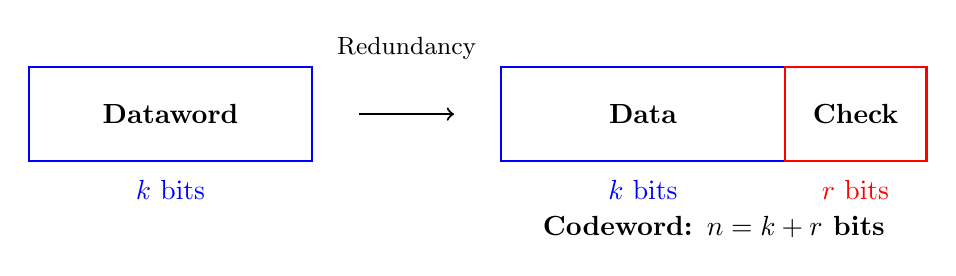
\begin{tikzpicture}[scale=1.2]
        % Dataword
        \draw[thick, blue] (0,1) rectangle (3,2);
        \node at (1.5,1.5) {\textbf{Dataword}};
        \node[blue] at (1.5,0.7) {$k$ bits};
        
        % Arrow
        \draw[->, thick] (3.5,1.5) -- (4.5,1.5);
        \node at (4,2.2) {\small Redundancy};
        
        % Codeword
        \draw[thick, blue] (5,1) rectangle (8,2);
        \draw[thick, red] (8,1) rectangle (9.5,2);
        \node at (6.5,1.5) {\textbf{Data}};
        \node at (8.75,1.5) {\textbf{Check}};
        \node[blue] at (6.5,0.7) {$k$ bits};
        \node[red] at (8.75,0.7) {$r$ bits};
        \node at (7.25,0.3) {\textbf{Codeword: $n = k + r$ bits}};
    \end{tikzpicture}
    \caption{Block coding adds redundancy bits to create error-detectable codewords}
    \label{fig:block_coding}
\end{figure}

Not all possible $n$-bit patterns are valid codewords - only specific combinations are allowed. When errors occur during transmission, the received pattern might not match any valid codeword, alerting us to corruption.

\subsubsection{Parity Bits: The Simplest Error Detection}
Parity\footnote{A number's parity is the property of being even or odd. In the context of error detection, it refers to the number of 1s in a binary representation.} checking is the most basic form of error detection. We add a single bit that makes the total number of 1s in the codeword either even (\textbf{even parity}) or odd (\textbf{odd parity}).

Let's see how even parity works with a 4-bit dataword:

\begin{table}[h]
\centering
\begin{tabular}{|c|c|c|c|c|c|}
\hline
\multicolumn{4}{|c|}{Dataword} & Parity & \multicolumn{1}{c|}{Total 1s} \\
\hline
$d_3$ & $d_2$ & $d_1$ & $d_0$ & $p$ & Count \\
\hline
0 & 0 & 0 & 0 & 0 & 0 (even) \\
0 & 0 & 0 & 1 & 1 & 2 (even) \\
0 & 0 & 1 & 0 & 1 & 2 (even) \\
0 & 0 & 1 & 1 & 0 & 2 (even) \\
0 & 1 & 0 & 0 & 1 & 2 (even) \\
\ldots & \ldots & \ldots & \ldots & \ldots & \ldots \\
\hline
\end{tabular}
\caption{Even parity ensures the total number of 1s is always even}
\label{tab:parity_example}
\end{table}

\textbf{Detection process:}
\begin{enumerate}
    \item Sender calculates parity bit and transmits dataword + parity
    \item Receiver counts all 1s in the received codeword
    \item If count is odd (for even parity), an error is detected
    \item If count is even, assume no error (though this isn't guaranteed!)
\end{enumerate}

\paragraph{Limitations of Simple Parity}
Simple parity can detect any \textbf{odd number} of bit errors (1, 3, 5, \ldots) but cannot detect \textbf{even numbers} of errors (2, 4, 6, \ldots). For example:

\begin{align*}
\text{Original:} \quad &1011\mathbf{0} \quad \text{(even parity, 3 ones total)}\\
\text{2-bit error:} \quad &1\mathbf{1}\mathbf{0}1\mathbf{0} \quad \text{(still even parity, 3 ones total)}
\end{align*}

The receiver would not detect this corruption! Simple parity operates on the principle of counting 1s, and when an even number of bits flip, the parity remains unchanged. In our example, the original codeword 10110 has three 1s (odd count), so with even parity we add a 0 to make it 101100 (four 1s total - even). After the 2-bit error occurs, 111100 still has four 1s (even count), so the parity check passes despite the data being corrupted.

This fundamental limitation occurs because parity checking uses modulo-2 arithmetic (XOR operations). When we flip an even number of bits, the XOR result remains the same:
\[
\text{bit}_1 \oplus \text{bit}_2 \oplus \ldots \oplus \text{bit}_n = \text{same result if even number of bits change}
\]

In fact, simple parity has a \textbf{50\% probability} of missing errors when multiple bits are corrupted - not much better than random guessing for multi-bit errors!

\paragraph{Two-Dimensional Parity}
To improve error detection, we can arrange data in a rectangular grid and add parity bits for both rows and columns:

\begin{figure}[h]
    \centering
    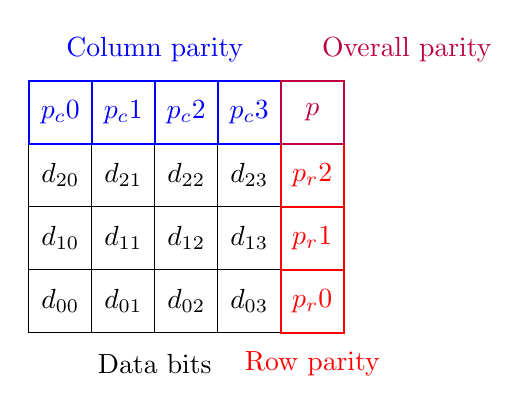
\begin{tikzpicture}[scale=0.8]
        % Data grid
        \foreach \i in {0,1,2} {
            \foreach \j in {0,1,2,3} {
                \draw (\j,\i) rectangle (\j+1,\i+1);
                \node at (\j+0.5,\i+0.5) {$d_{\i\j}$};
            }
        }
        
        % Row parity
        \foreach \i in {0,1,2} {
            \draw[red, thick] (4,\i) rectangle (5,\i+1);
            \node[red] at (4.5,\i+0.5) {$p_r\i$};
        }
        
        % Column parity
        \foreach \j in {0,1,2,3} {
            \draw[blue, thick] (\j,3) rectangle (\j+1,4);
            \node[blue] at (\j+0.5,3.5) {$p_c\j$};
        }
        
        \draw[purple, thick] (4,3) rectangle (5,4);
        \node[purple] at (4.5,3.5) {$p$};
        
        % Labels
        \node at (2,-0.5) {Data bits};
        \node[red] at (4.5,-0.5) {Row parity};
        \node[blue] at (2,4.5) {Column parity};
        \node[purple] at (6,4.5) {Overall parity};
    \end{tikzpicture}
    \caption{Two-dimensional parity can detect and sometimes correct single-bit errors}
    \label{fig:2d_parity}
\end{figure}

Two-dimensional parity can:
\begin{itemize}
    \item \textbf{Detect} most patterns of 2-bit and 3-bit errors
    \item \textbf{Locate and correct} single-bit errors
    \item Still fail for certain 4-bit error patterns
\end{itemize}

\subsubsection{Cyclic Redundancy Check (CRC)}
While parity bits are simple, they're not very powerful. For better error detection, we turn to Cyclic Redundancy Check (CRC) - this is actually being used in real-life networks.

CRC is based on \textbf{polynomial arithmetic} over finite fields. Don't panic! The math is elegant once you understand the pattern.

\paragraph{The Big Idea}
Think of your data as coefficients of a polynomial. For example, the bits \texttt{1101} represent:
\[
1 \cdot x^3 + 1 \cdot x^2 + 0 \cdot x^1 + 1 \cdot x^0 = x^3 + x^2 + 1
\]

CRC works by:
\begin{enumerate}
    \item Treating data as a polynomial $M(x)$
    \item Choosing a \textbf{generator polynomial} $G(x)$
    \item Computing the remainder when $x^r \cdot M(x)$ is divided by $G(x)$
    \item Appending this remainder as the CRC bits
\end{enumerate}

\begin{importantblock}
    If no errors occur, the received codeword will be perfectly divisible by $G(x)$. If division leaves a remainder, we know errors have occurred.
\end{importantblock}

\begin{noteblock}
    CRC-32 (used in Ethernet and many other protocols) has a 32-bit check sequence and can detect virtually all error patterns in practice. The probability of an undetected error is approximately $2^{-32} \approx 2.3 \times 10^{-10}$ - incredibly small!
\end{noteblock}

TODO: CRC calculation details\ldots
% flow control
\input{sections/datalink/4_flow_control.tex}
% link management
\input{sections/datalink/5_link_management.tex}
% protocols
\input{sections/datalink/6_protocols.tex}
